\section{Jets reconstruction and identification}\label{sec:jets}

Jets are the experimental signature of quarks and gluons produced in high energy physics processes. They arise from the hadronization of partons, which forms collimated sprays of particles. In this section the jet reconstruction techniques used in CMS are described.

\subsection{Jet reconstruction in CMS}

The majority of physics analyses involving jets in the final state make use of Particle Flow jets. The PF jets are reconstructed using the technique described in Sec.~\ref{sec:PF}, clustering all particles reconstructed with the PF algorithm, without any distinction of type and energy threshold. This method allows a remarkable improvement in the jet momentum and spatial resolution with respect to the calorimeter jets, which are instead reconstructed using solely the information from the calorimeters. Indeed the use of the tracker information provides a better \pt resolution for the charged particles belonging to jets\footnote{On average, the typical jet energy fractions carried by charged particles, photons and neutral particles are 65\%, 25\% and 10\%, respectively at low \pt. For higher jet \pt the energy fraction carried by photons and neutral hadrons increases.}. 

Jets are defined through sequential, iterative clustering algorithms that combine the four-momenta of input particles until certain conditions are satisfied and jets are formed~\cite{Salam:2009jx}. Several algorithms are available for jet clustering, characterized by different features. From a theoretical point of view, an ideal jet clustering algorithm should fulfil the following requirements~\cite{Blazey:2000qt}:
\begin{itemize}
\item \emph{Infrared safety}: infrared singularities should not appear in the perturbative calculations and the solutions of the algorithm should be insensitive to soft radiation in the event;
\item \emph{Collinear safety}: collinear singularities should not appear in the perturbative calculations and jets should be insensitive to collinear radiation in the event;
\item \emph{Invariance under boosts}: the solutions of the algorithm should be the same independently of boosts in the longitudinal direction. This is particularly important for hadron colliders, where the centre-of-mass of the individual parton-parton collisions is typically boosted along the beam direction;
\item \emph{Order independence}: the algorithm should find the same jets at parton, particle and detector level;
\item \emph{Straightforward implementation}: the algorithm should be straightforward to implement in perturbative calculations.
\end{itemize}
The ideal algorithm should also follow some experimental attributes. Among them, the performance of the algorithm should be as independent as possible of the detector that provides the data, the algorithm should not amplify the inevitable effects of resolution smearing and angle bias and should not be strongly affected by pile-up and high beam luminosities. Furthermore, the algorithm should be easy to implement, efficient to identify all possible jet candidates and should keep the necessary computing resources at an acceptable level.

Two main classes of jet clustering algorithms may be defined. The first one consists in the ``cone'' recombination, where jets are reconstructed associating together particles whose trajectories lie within a cone of radius $\Delta R$ in the $\eta$--$\phi$ plane. An example of this approach is the SISCone algorithm. The second class of algorithms uses the sequential recombination scheme, that iteratively recombine the closest pair of particles according to some distance measure.

The standard algorithms used by CMS are the $k_t$, anti-$k_t$ and \emph{Cambridge Aachen} (CA) algorithms, which belong to the sequential recombination class.
The $k_t$, anti-$k_t$ and CA algorithms are infrared and collinear safe algorithms characterized by the introduction of two definitions of distance: $d_{ij}$, the distance between the two objects $i$ and $j$, and $d_{iB}$, the distance between the object $i$ and the beam. These distances are defined by the following equations:
\begin{equation}\label{eq:jetalgo}
\begin{split}
d_{ij} &= min\left(k_{ti}^{2p}, k_{tj}^{2p} \right) \frac{\Delta_{ij}^2}{R^2} \quad,\\
d_{iB} &= k_{ti}^{2p} \quad,
\end{split}
\end{equation}
where $\Delta_{ij}^2 = (y_i - y_j)^2 + (\phi_i - \phi_j)^2$ and $k_{ti}$, $y_i$ and $\phi_i$ are the transverse momentum, rapidity and azimuthal angle of the particle $i$, respectively. In these formulas, $R$ represents the radial parameter and $p$ is a parameter that is 1 for $k_t$, 0 for CA and $-1$ for anti-$k_t$ algorithm. The algorithm proceeds as follows:
\begin{itemize}
\item the distances $d_{ij}$ are calculated for all pairs of particles $i,j$ and the distances $d_{iB}$ are calculated for each particle $i$, according to Eq.~\eqref{eq:jetalgo};
\item the smallest distance, which could be either of type $d_{ij}$ or $d_{iB}$, is identified;
\item if the smallest distance is a $d_{ij}$, the particles $i$ and $j$ are combined into a single new particle summing their four-momenta and the algorithm restarts from the first step;
\item otherwise, if it is a $d_{iB}$, $i$ is declared to be a final state jet and the algorithm returns to the first step;
\item the procedure is repeated until no particles are left.
\end{itemize}

The physical difference between the three algorithms is the momentum weighting. For the $k_t$ algorithm, the weighting proportional to $k_t^2$ implies that jets are reconstructed starting from particles with low transverse momentum. Moreover, this algorithm produces jets with irregular borders, thereby complicating the correction for effects such as pile-up. For the CA algorithm there is no transverse momentum weighting and particles are merged following just an angular approach, based on the distance $\Delta_{ij}$. Also this algorithm leads to jets with irregular borders. Finally, the anti-$k_t$ algorithm uses a weighting proportional to $1/k_t^2$, favouring the merging of high transverse momentum particles. In this case the jets grow around particles with highest transverse momenta and jets have a circular shape. 

Jets reconstructed with different algorithms starting from the same set of simulated particles are shown in Fig.~\ref{fig:jets}. All the analyses presented in Chapters~\ref{chap4}, \ref{chap5} and \ref{chap6} make use of the sequential recombination scheme. In particular the anti-$k_t$ algorithm is used, with $R=0.5$ and $R=0.4$ for analyses at 8\TeV and 13\TeV, respectively.

\begin{figure}[htb]
\centering
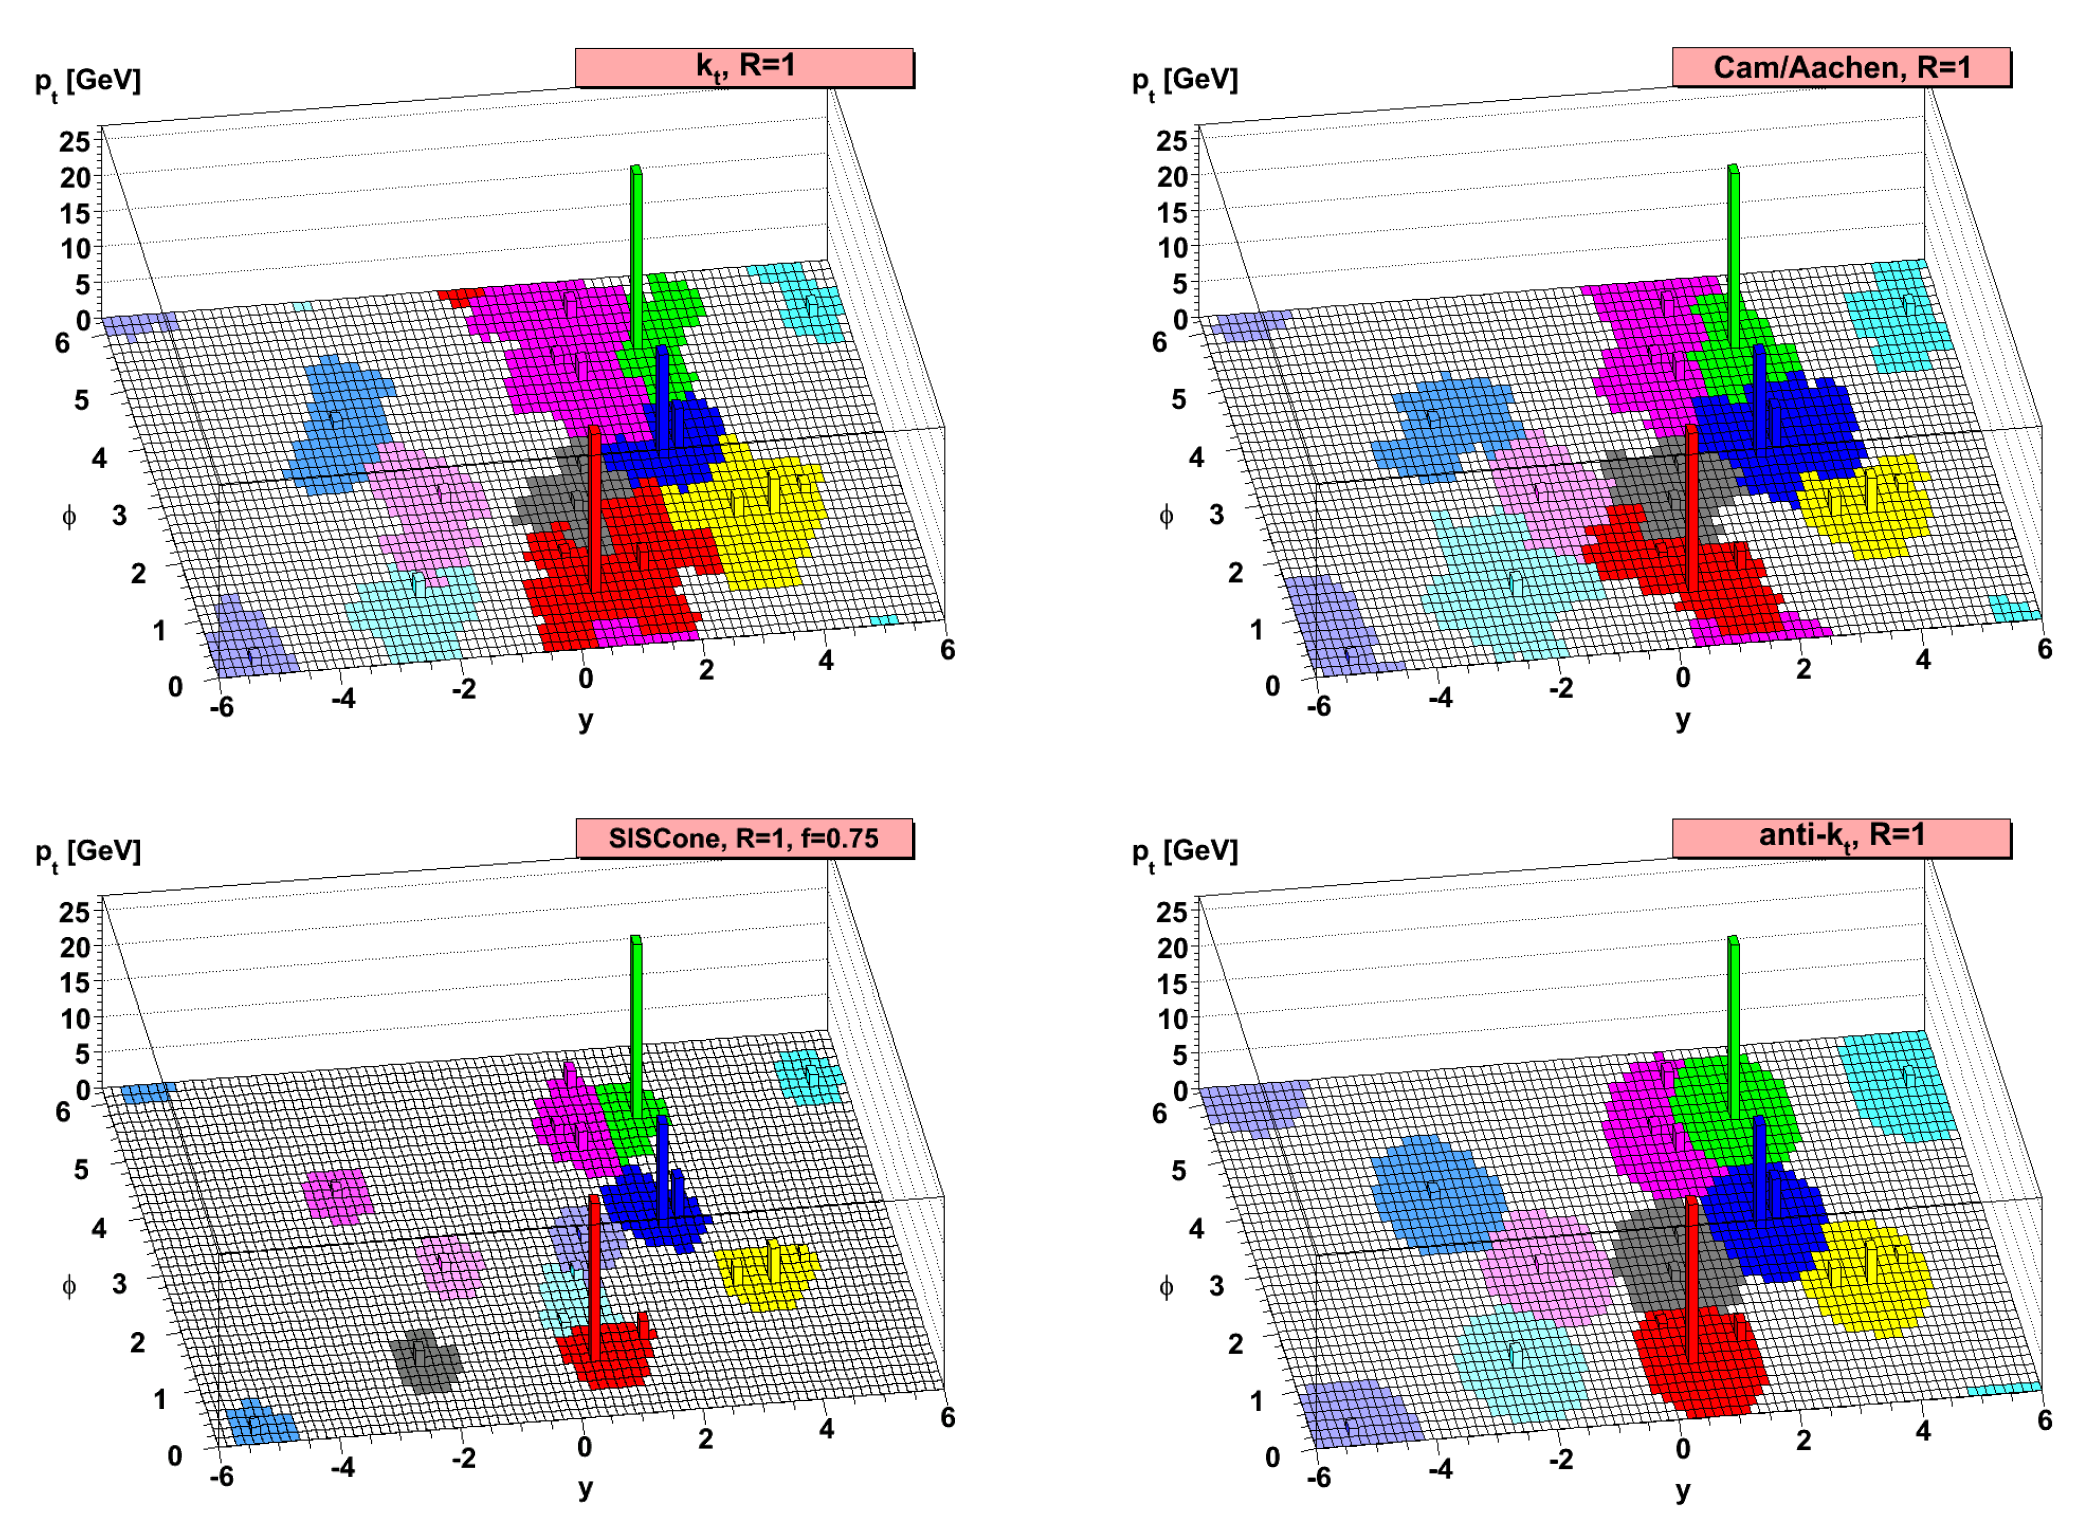
\includegraphics[width=0.7\textwidth]{images/jets.png}
\caption{Jets reconstructed with different algorithms starting from the same set of simulated particles. The jets reconstructed with the sequential recombination algorithms described in the text are shown, as well as with the SISCone algorithm.}\label{fig:jets}
\end{figure}

\subsection{Jet energy correction}\label{sec:jec}

The purpose of jet energy correction is to relate, on average, the jet energy measured in the detector to the true energy of the corresponding final state particle or parton jet. The latter is obtained in simulation by clustering all stable particles, i.e. with $c\tau > 1$\,cm, produced in the event excluding neutrinos, using the same clustering algorithm as for jets in the detector. A mismatch is mainly ascribable to the nonuniform and nonlinear response of the CMS calorimeters, electronics noise and pile-up. For this reason, CMS has developed a sequential procedure to calculate and apply the \emph{jet energy corrections} (JEC)~\cite{Chatrchyan:2011ds}.

The correction is applied as a multiplicative factor ($\mathcal{C}$) to each component of the raw jet four-momentum $p_\mu^\mathrm{raw}$ (components are indexed by $\mu$ in the following):
\begin{equation}
p_\mu^\mathrm{cor} = \mathcal{C}\cdot p_\mu^\mathrm{raw} \quad,
\end{equation}
where $p_\mu^\mathrm{cor}$ is the corrected jet four-momentum. The correction factor is composed of the offset correction $C_\mathrm{offset}$, the MC calibration factor $C_\mathrm{MC}$, and the residual calibrations $C_\mathrm{rel}$ and $C_\mathrm{abs}$ for the relative and absolute energy scales, respectively. The offset correction removes the extra energy due to noise and pile-up, and the MC correction removes the bulk of the nonuniformity in $\eta$ and the nonlinearity in \pt. Finally, the residual corrections account for the small differences between data and simulation. The various components are applied in sequence as described by the equation below:
\begin{equation}
\mathcal{C} = C_\mathrm{offset}(\pt^\mathrm{raw}) \cdot C_\mathrm{MC}(\pt',\eta) \cdot C_\mathrm{rel}(\eta) \cdot C_\mathrm{abs}(\pt'') \quad ,
\end{equation}
where $\pt'$ is the jet \pt after applying the offset correction and $\pt''$ is the jet \pt after applying all previous corrections. Each component is briefly described in the following sections.

\subsubsection{Offset correction}
 
The offset correction purpose is to estimate and subtract the average energy contribution that is not associated with the hard scattering in the event. The approach followed for the estimation of the offset correction is known as \emph{Jet Area Method}~\cite{Cacciari:2007fd}. For each event, an average \pt-density per unit area, $\rho$, is estimated, characterizing the soft jet activity. This \pt-density represents the combination of underlying event, electronics noise and pile-up effects. 
The two latter components contaminate the hard jet energy measurement and need to be
corrected for with the offset correction. The key element for this approach is the jet area $A_j$.
A very large number of infinitely soft four-momentum vectors (soft enough not to change the properties of the true jets) are artificially added in the event and clustered by the jet algorithm together with the true jet components. The extent of the region in the $\eta$--$\phi$ space occupied by the soft particles clustered in each jet defines the active jet area. The \pt-density $\rho$ is calculated with the $k_t$ algorithm with a distance parameter $R=0.6$. The quantity $\rho$ is estimated event by event as the median of the distribution of the variable $p_{\mathrm{T}j}/A_j$, where $j$ runs over all jets in the event, and is not sensitive to the presence of hard jets. At detector level, the measured density $\rho$ is the convolution of the true particle-level activity (underlying event, pile-up) with the detector response to the various particle types. Therefore, the event-by-event and jet-by-jet offset correction can be defined as:

\begin{equation}
C_\mathrm{offset}(\pt^\mathrm{raw},A_j,\rho) = 1 - \frac{\left( \rho - \langle\rho_\mathrm{UE}\rangle \right)\cdot A_j}{\pt^\mathrm{raw}}\quad .
\end{equation}

\noindent In the formula above, $\langle\rho_\mathrm{UE}\rangle$ represents the average \pt-density component due to underlying event and electronics noise, measured in events with exactly one reconstructed primary vertex, i.e. no pile-up.

An additional pile-up subtraction method that is used in CMS is called \emph{Charged Hadron Subtraction} (CHS). This method makes use of PF jets and exploits the excellent CMS tracking capabilities to identify and remove charged hadrons inside jets that are known to originate from pile-up vertices. This is a particle-by-particle method that is applied to jets before calculating the offset correction.

\subsubsection{MC calibration correction}

The MC calibration is based on simulation and corrects the energy of the reconstructed jets such that it is equal on average to the energy of the generated jets. In order to evaluate this correction, simulated QCD events are generated and then processed through the CMS detector simulation based on the \textsc{Geant4} software~\cite{Agostinelli:2002hh}. The jet reconstruction in simulation is identical to the one applied to data. Each reconstructed jet is spatially matched, in the $\eta$--$\phi$ space, to a generated jet by requiring $\Delta R < 0.25$. In each bin of the generated jet transverse momentum $\pt^\mathrm{gen}$, the response variable $\mathcal{R}=\pt^\mathrm{reco}/\pt^\mathrm{gen}$ and the reconstructed jet transverse momentum $\pt^\mathrm{reco}$, are saved. The average correction in each bin is therefore defined as:

\begin{equation}
C_\mathrm{MC}(\pt^\mathrm{reco}) = \frac{1}{\langle \mathcal{R} \rangle} \quad,
\end{equation}

\noindent and is expressed as a function of the average reconstructed jet \pt, $\langle \pt^\mathrm{reco} \rangle$.

\subsubsection{Relative jet energy scale}

The goal of the relative jet energy scale correction is to make the jet response flat versus $\eta$. This is achieved by employing a Tag and Probe technique, selecting dijet events in data. The size of this residual correction is of the order of 2--3\% in the central $\eta$ region, while it goes up to about 10\% in the forward region.

\subsubsection{Absolute jet energy scale}

The goal of the absolute jet energy scale correction is to make the jet response flat versus \pt. The absolute jet energy response is measured in the reference region $|\eta|<1.3$ with the \emph{Missing Transverse Energy Projection Fraction} (MPF) method~\cite{Abbott:1998xw}, using $\gamma+\mathrm{jets}$ and Z$+\mathrm{jets}$ events. This method is used to estimate the absolute jet energy correction and is based on the fact that $\gamma+\mathrm{jets}$ and Z$+\mathrm{jets}$ events have no intrinsic \MET and that, at parton level, the $\gamma$ and Z boson are perfectly balanced by the hadronic recoil in the transverse plane (see Sec.~\ref{sec:metscale}).

\subsubsection{Jet energy uncertainties}

The uncertainties in the jet energy estimation arise from several sources. Generally these can be categorized as follows:
\begin{itemize}
\item physics modelling in MC such as showering, underlying event, etc.;
\item MC modelling of true detector response and properties;
\item potential biases in the methodologies used to estimate the corrections.
\end{itemize}
The sources are combined in different groups: absolute scale, relative scale, pile-up, jet flavor and time stability. In Fig.~\ref{fig:JECunc} the effect of each group of uncertainties is shown together with the total uncertainty obtained summing all sources in quadrature, both as a function of $\eta$ and \pt. The pile-up uncertainty dominates for low values of the jet \pt while the relative and absolute uncertainties are more important in the high \pt region.

\begin{figure}[htb]
\centering
\subfigure{
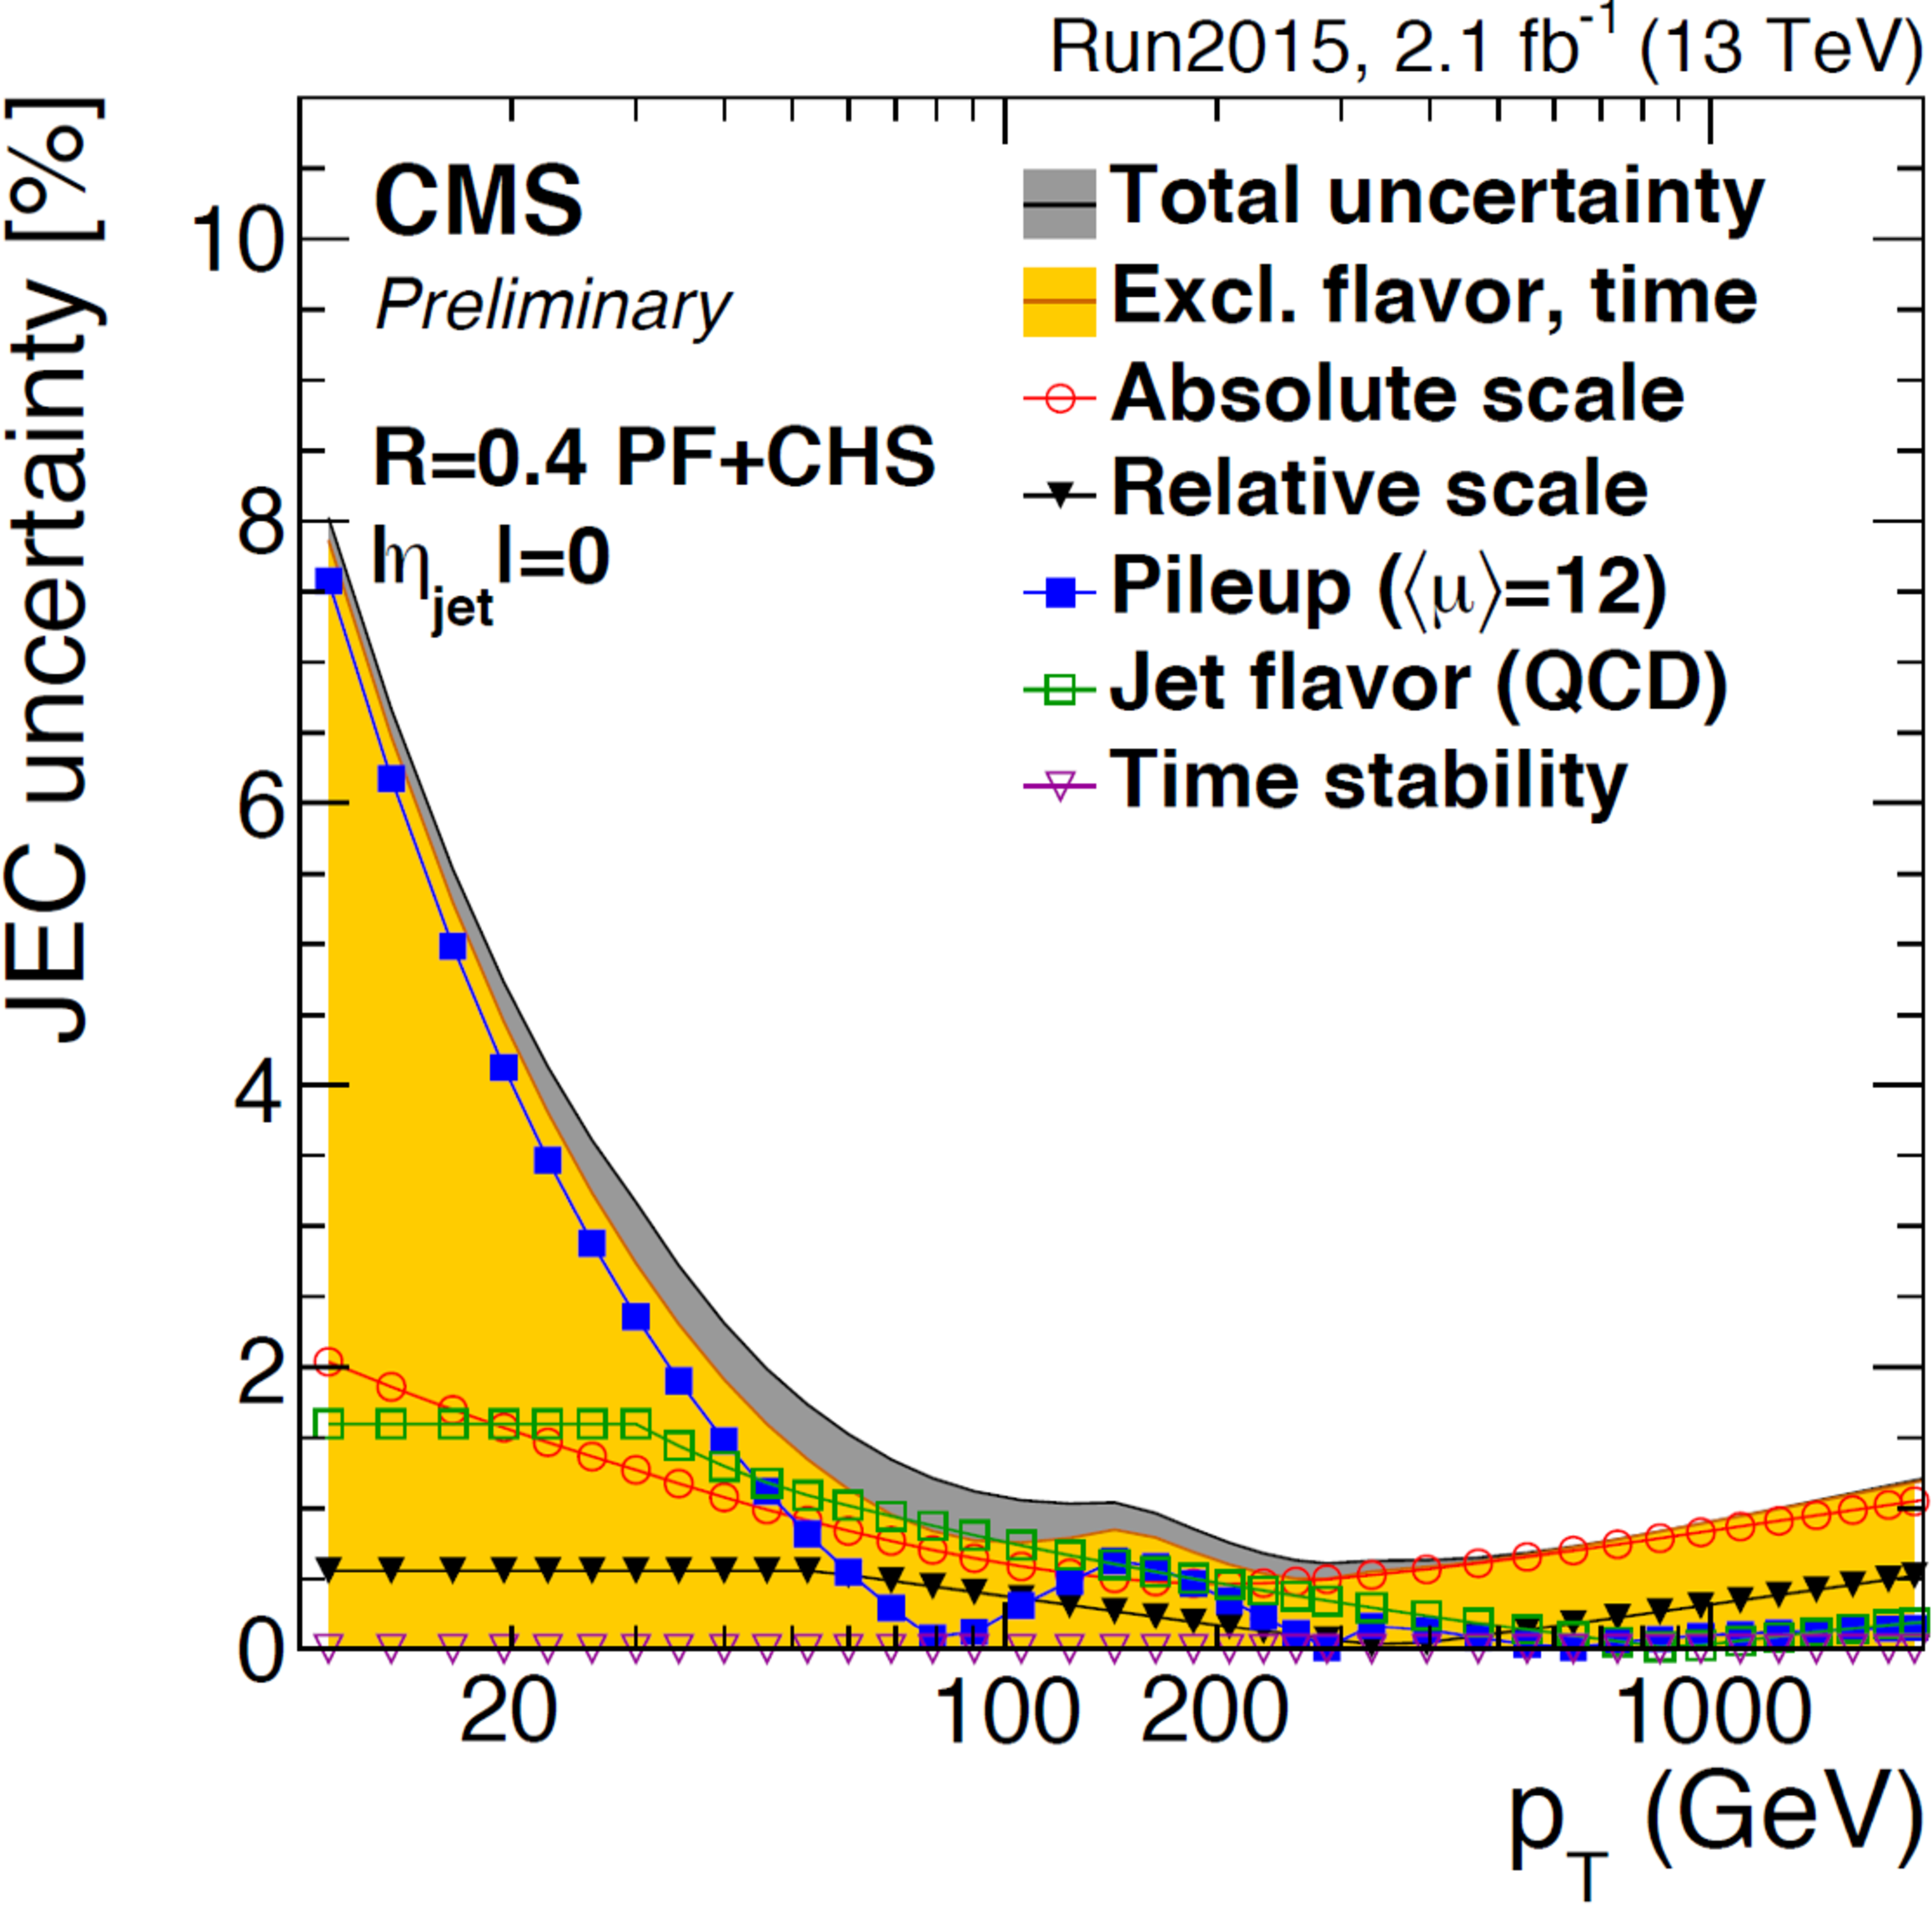
\includegraphics[width=0.45\textwidth]{images/jetUncPt.pdf}
}
\subfigure{
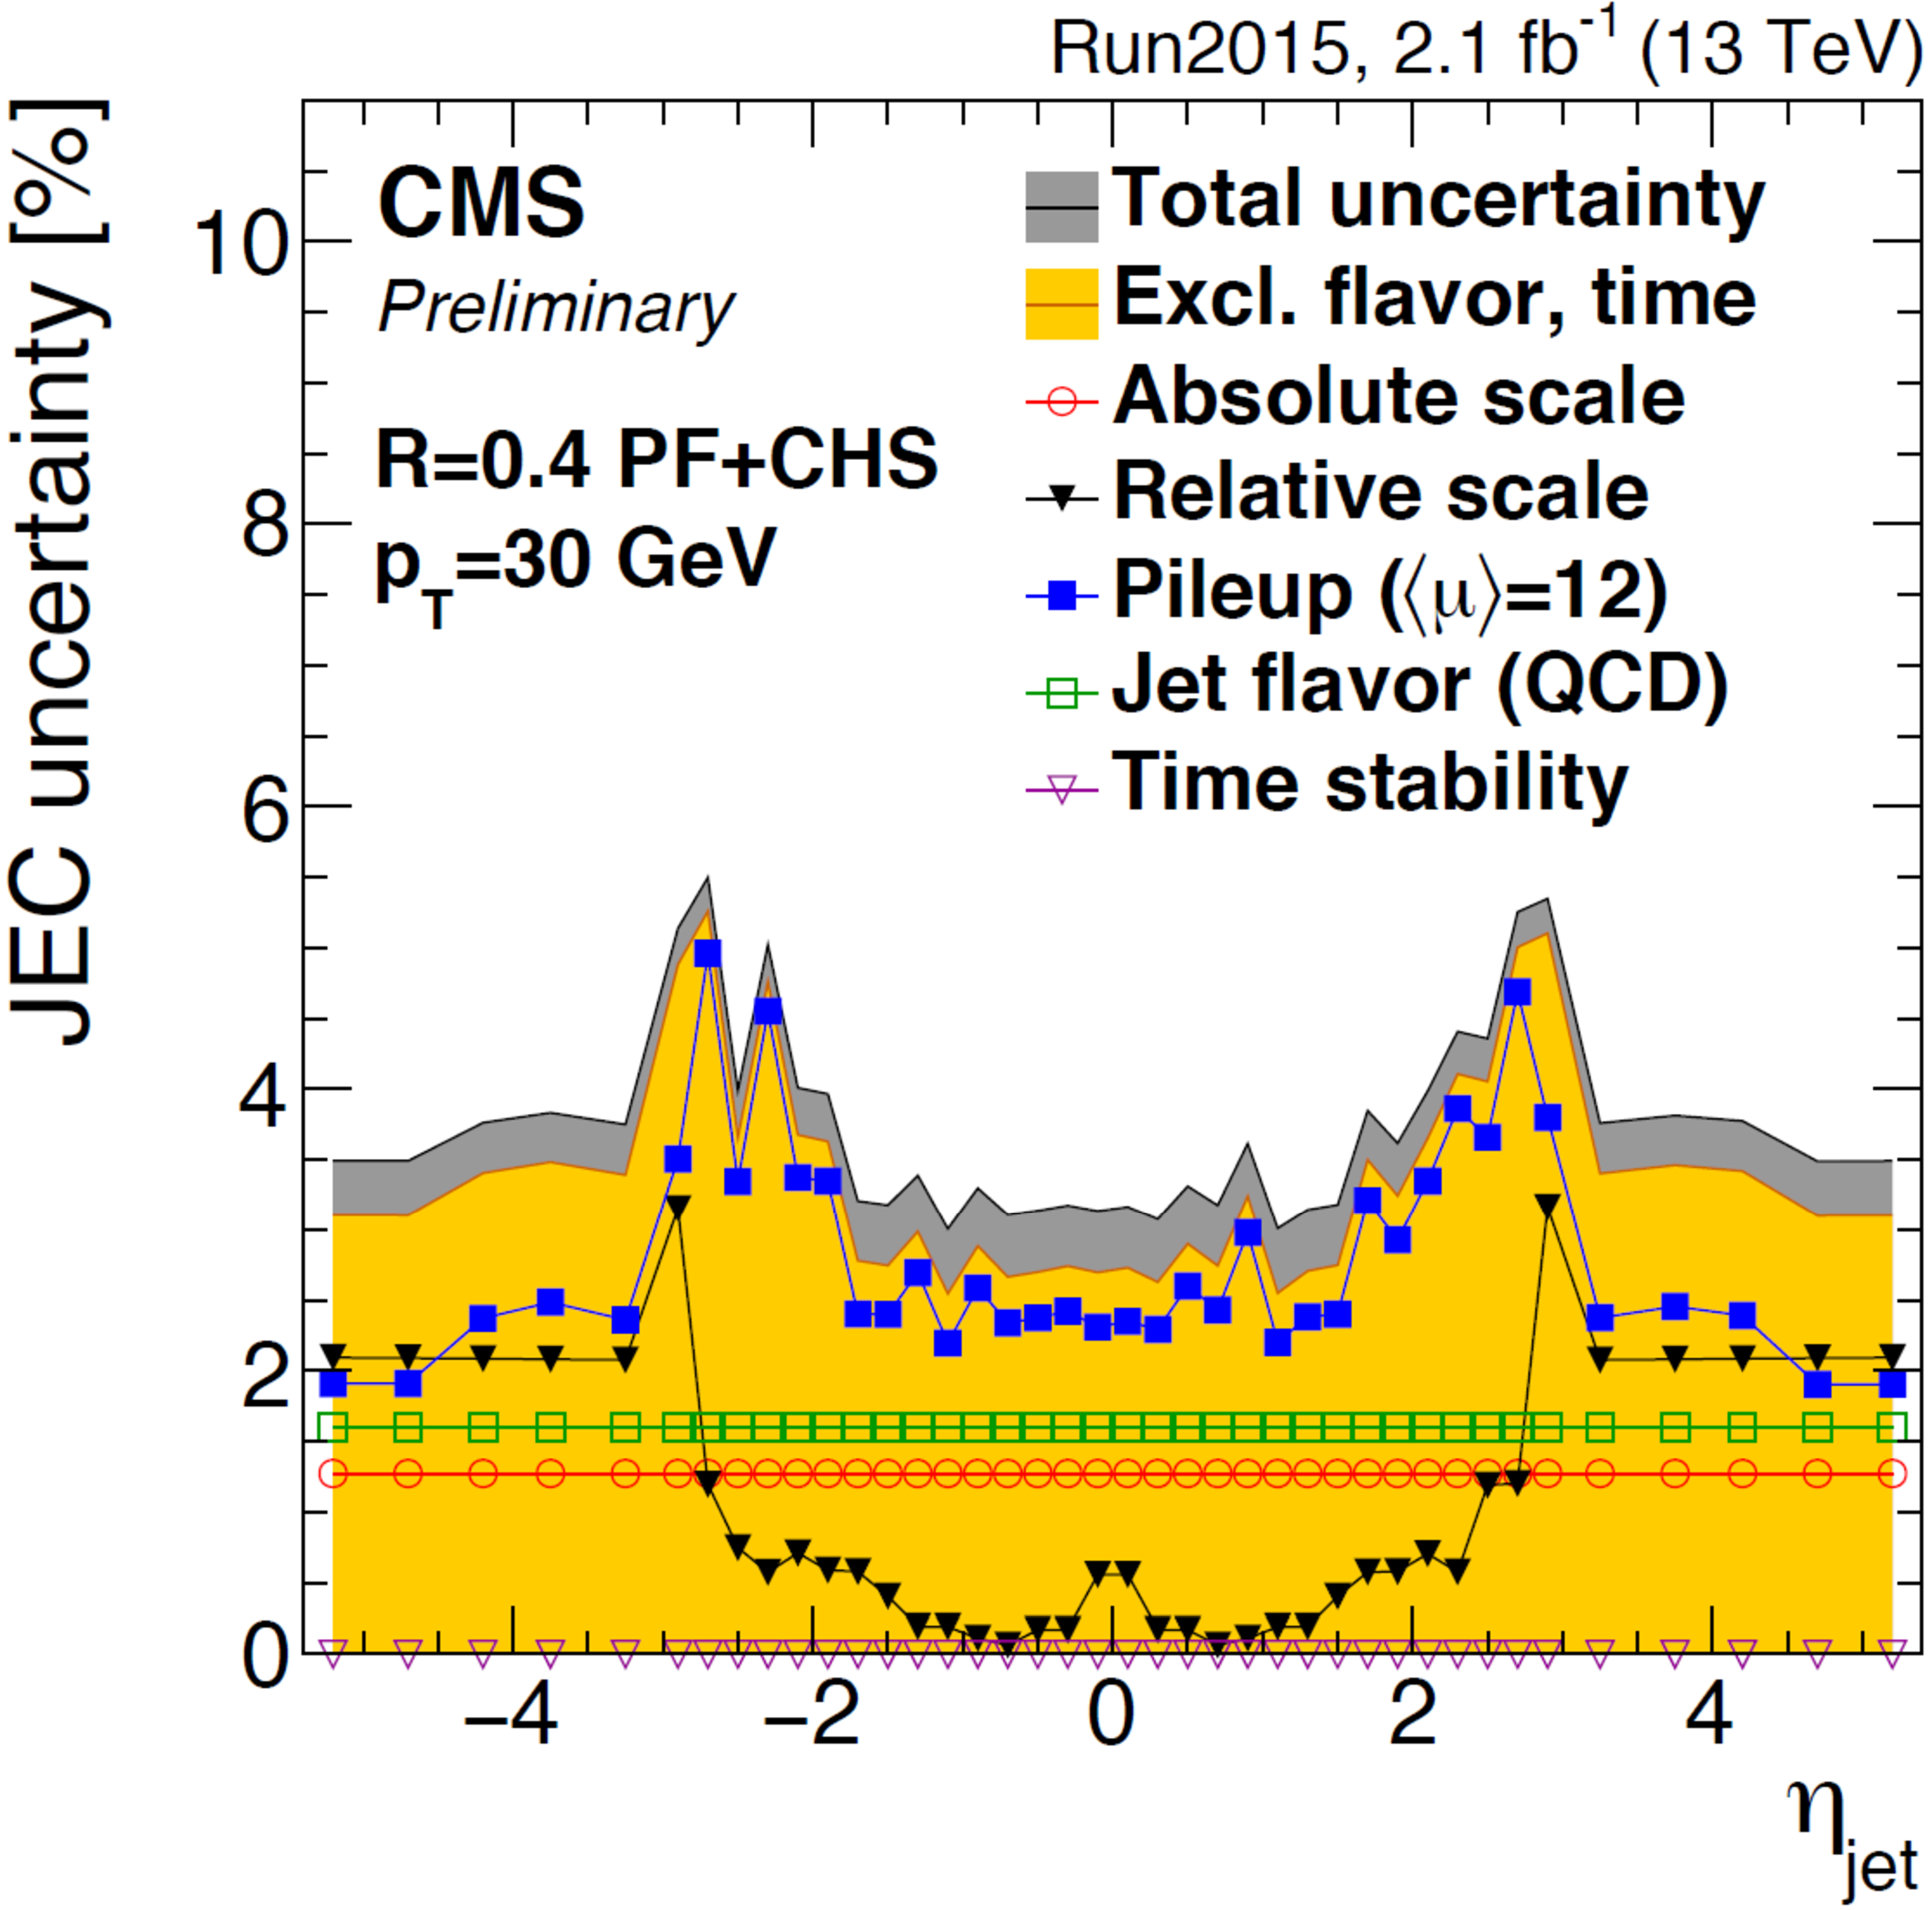
\includegraphics[width=0.45\textwidth]{images/jetUncEta.pdf}
}
\caption{JEC uncertainties as a function of \pt (left) for jets reconstructed with $\eta=0$ and as a function of $\eta$ (right) for jets with $\pt=30$\,\GeV. All jets are reconstructed with the PF technique and using the anti-$k_t$ algorithm with $R=0.4$, after applying the CHS correction. Results are based on $2.1$\,\ifb of data collected at 13\,\TeV.}\label{fig:JECunc}
\end{figure}

\subsubsection{Jet energy resolution}
Measurements show that the jet energy resolution (JER) in data is worse than in simulation, therefore the simulated jets need to undergo a smearing procedure in order to have a better description of the data. 

Reconstructed jets in simulated events are corrected for the jet energy resolution using a two step procedure. In the first step, the reconstructed jet \pt is scaled for the observed \pt difference between reconstructed and generated jets. This method only works for reconstructed jets that are well matched to generated jets, where the matching is based on $\Delta R$ and $\Delta \pt$ requirements. In the second step, a gaussian smearing of the \pt distribution of the reconstructed jet is applied in order to obtain the desired resolution. For reconstructed jets that do not fulfil the matching requirement to generated jets, only the second step is applied.

\subsection{Jet identification}\label{sec:jetID}

Some basic quality criteria for jets may be required in order to avoid fake jets to be used, which can originate from noisy calorimetric cells or electronics noise. These criteria are collectively called \emph{jet identification} (or Jet ID) and allow the rejection of badly reconstructed or noise jets while maintaining a very large fraction (about 99\%) of real jets. Two working points are defined, loose and tight, based on requirements on the hadron and electromagnetic components of the jet. The sets of criteria are illustrated in Table~\ref{tab:jetID} for PF jets with $|\eta|<3$. For $3<|\eta|<5$ the neutral electromagnetic fraction is required to be below $0.90$ and the neutral multiplicity larger than $10$ for both working points.

\begin{table}[htb]
\centering
\caption{Jet identification criteria for the loose and tight working points. The requirements are based on PF jets with $|\eta|<3$ for the neutral component and $|\eta|<2.4$ for the charged component.}\label{tab:jetID}
\begin{tabular}{l c c}
\toprule
Variable & Loose working point & Tight working point \\
\midrule
\pt & $>10$\GeV & $>10$\GeV \\
Number of constituents & $>1$ & $>1$ \\
Charged hadron fraction & $>0$ & $>0$ \\
Neutral hadron fraction & $<0.99$ & $<0.90$ \\
Charged multiplicity & $>0$ & $>0$ \\
Charged electromagnetic fraction & $<0.99$ & $<0.90$ \\
Neutral electromagnetic fraction & $<0.99$ & $<0.90$ \\
\bottomrule
\end{tabular}
\end{table}

An additional algorithm may be used to reduce the incidence of jets originating from pile-up. These jets arise mainly from the overlap of multiple low-\pt jets originated from different interaction vertices, which combine forming single high-\pt jets. The pile-up jet identification algorithm makes use of both vertex information, exploiting the charged component of the jet, and jet shape information to identify jets ascribable to pile-up.
